%%%%%%%%%%%%%%%%%%%%%%%%%%%%%%%%%%%%%%%%%
% Short Sectioned Assignment
% LaTeX Template
% Version 1.0 (5/5/12)
%
% This template has been downloaded from:
% http://www.LaTeXTemplates.com
%
% Original author:
% Frits Wenneker (http://www.howtotex.com)
%
% License:
% CC BY-NC-SA 3.0 (http://creativecommons.org/licenses/by-nc-sa/3.0/)
%
%%%%%%%%%%%%%%%%%%%%%%%%%%%%%%%%%%%%%%%%%

%----------------------------------------------------------------------------------------
%	PACKAGES AND OTHER DOCUMENT CONFIGURATIONS
%----------------------------------------------------------------------------------------

\documentclass[paper=a4, fontsize=11pt]{article} % A4 paper and 11pt font size

\usepackage[T1]{fontenc} % Use 8-bit encoding that has 256 glyphs
%\usepackage{fourier} % Use the Adobe Utopia font for the document - comment this line to return to the LaTeX default
\usepackage[english]{babel} % English language/hyphenation
\usepackage{amsmath,amsfonts,amsthm} % Math packages

\usepackage{sectsty} % Allows customizing section commands
\allsectionsfont{\centering \normalfont\scshape} % Make all sections centered, the default font and small caps

\usepackage{fancyhdr} % Custom headers and footers
\pagestyle{fancyplain} % Makes all pages in the document conform to the custom headers and footers
\fancyhead{} % No page header - if you want one, create it in the same way as the footers below
\fancyfoot[L]{} % Empty left footer
\fancyfoot[C]{} % Empty center footer
\fancyfoot[R]{\thepage} % Page numbering for right footer
\renewcommand{\headrulewidth}{0pt} % Remove header underlines
\renewcommand{\footrulewidth}{0pt} % Remove footer underlines
\setlength{\headheight}{13.6pt} % Customize the height of the header

\numberwithin{equation}{section} % Number equations within sections (i.e. 1.1, 1.2, 2.1, 2.2 instead of 1, 2, 3, 4)
\numberwithin{figure}{section} % Number figures within sections (i.e. 1.1, 1.2, 2.1, 2.2 instead of 1, 2, 3, 4)
\numberwithin{table}{section} % Number tables within sections (i.e. 1.1, 1.2, 2.1, 2.2 instead of 1, 2, 3, 4)

\setlength\parindent{0pt} % Removes all indentation from paragraphs - comment this line for an assignment with lots of text

\usepackage{hyperref}
\usepackage{geometry}

\usepackage{graphicx}
\usepackage{multirow}
\usepackage{wrapfig}
\usepackage{amssymb}% http://ctan.org/pkg/amssymb
\usepackage{pifont}% http://ctan.org/pkg/pifont

%----------------------------------------------------------------------------------------
%	TITLE SECTION
%----------------------------------------------------------------------------------------

\begin{document}

\title{Charlie's notes}

\maketitle
%----------------------------------------------------------------------------------------
%	PROBLEM 1
%----------------------------------------------------------------------------------------

\section{CS31310 - Agile}




%------------------------------------------------

\section{CS36110 - Machine Learning}


%------------------------------------------------

\section{CS34110 - Computer Vision}

\subsection{November 20: Motion Models}

\textbf{Modelling Change \& Tracking}

\paragraph{Motion:}
\begin{itemize}
\item Background Subtraction
\item Optical Flow
\end{itemize}

\paragraph{Mixture of Gaussians (MoG):}
\begin{itemize}
\item Robust to noise
\item Handles shadows ok
\item Common first step
\end{itemize}

\subsubsection{Tracking: Modelling change}

\paragraph{Video:}
\begin{itemize}
\item detections in each frame
\item detections are noisy \& computationally expensive
\item tracking mitigates both issues
\end{itemize}

Noise can occur if the camera on a robot/car is moving up/down

\subsubsection{A general framework for tracking}

\paragraph{Recursively:}
\begin{itemize}
\item An idea about how something will change (\textit{Model})
\item Make a prediction (\textit{Predict})
\item See what happens (\textit{Measure})
\item Update model (\textit{Update})
\end{itemize}

\paragraph{Advantages:}
\begin{itemize}
\item Smooths the data 
	\begin{itemize}
	\item	estimate location upon predictions  \& the measurement
	\end{itemize}
\item Constrains search
	\begin{itemize}
	\item start looking for target in the location it was last seen		
	\end{itemize}
\end{itemize}

\subsubsection{Kalman Filter}

\begin{itemize}
\item Like predict, measure, update from earlier
\item Useful for tracking
\item Copes well with missing information (occlusions) 
\end{itemize}

\begin{figure}[h]
    \centering
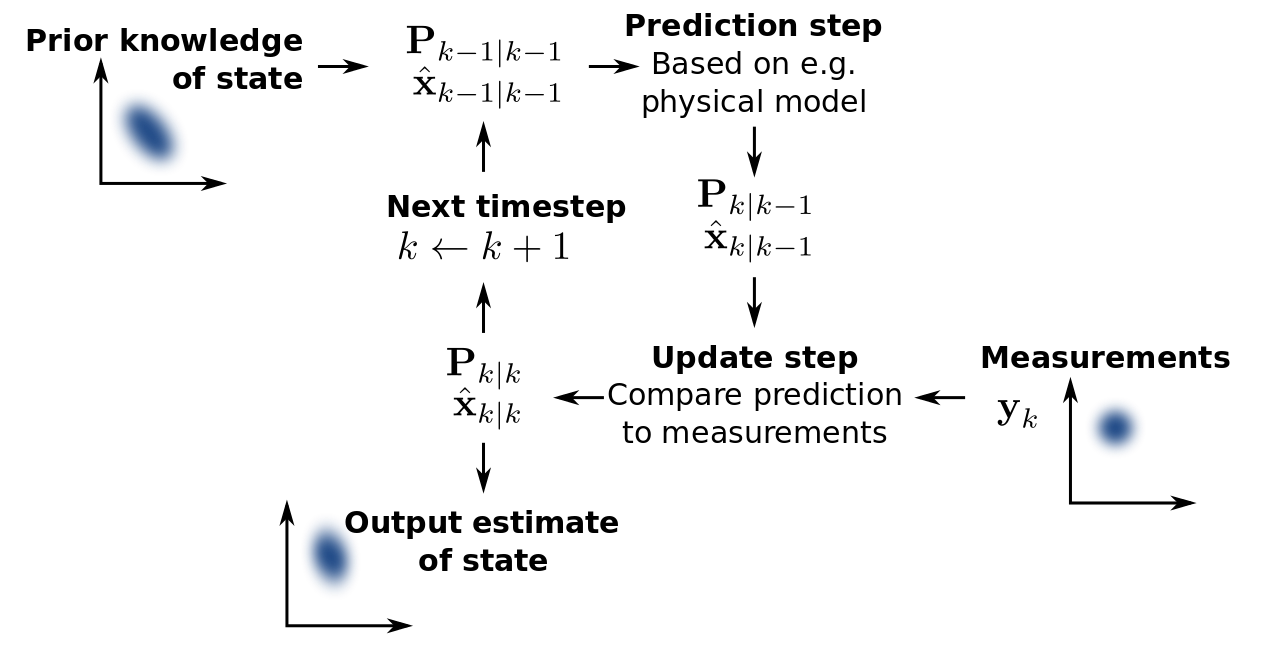
\includegraphics[scale=0.3]{images/kalman}
\caption{Sourced from Wikipedia}
    \label{fig:kalman}
\end{figure}

\begin{center}

\begin{tabular}{| c  c  c  c | c |}
\hline
Background subtraction & $\rightarrow$ & Pixels grouped into objects & $\rightarrow$ & \multirow{3}{4em}{Tracker} \\ 
Sparse Optical Flow &  $\rightarrow$  & Features grouped into objects &  $\rightarrow$  & \\ 
Face Detection &   $\rightarrow$   &  $\rightarrow$  &   $\rightarrow$   & \\ \hline

\end{tabular}
\end{center}

\paragraph{Use Kalman to smooth any measurement}
\begin{itemize}
\item X,Y location
\item size
\item colour
\end{itemize}

\textbf{See also:} Particle filtering: works with combining and splitting objects (e.g. people holding hands, then letting go)

\textbf{Hannah's video: } \url{https://www.youtube.com/watch?v=NYdwpX1a7-Y}

\subsubsection{Mean Shift}

\begin{wrapfigure}{r}{0.5\textwidth}
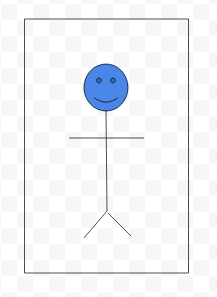
\includegraphics[scale = 0.5]{images/mean_shift}
\end{wrapfigure}

Computer the mean of the data within the window

Shift the window to the mean every time

\paragraph{Notes:}
\begin{itemize}
\item Changes size - can use CAM-Shift to mitigate?
\item Lighting change - not really, gradually changes mean over time
\item If it picks up something you're not looking for, will slowly drift off
\end{itemize}

\subsubsection{Problems with Tracking}

\begin{itemize}
\item Initialisation (what are you tracking?)
\item Having more than 1 item to track
\item Losing target due to motion / occlusion
\item Losing target due to appearance change
\end{itemize}

Usually initialise from a detector of some sort

\textbf{Useful speed up for detectors \& accuracy}

Look into: TLD: Tracking Learning Description

\subsubsection{Closing note}

Vision Systems tend to have multiple layers

Tracking is extremely common in anything which deals with change.

\paragraph{HOG for example, has several layers:}
\begin{itemize}
\item 2D filters
\item Tangent
\item Histogram
\item Superimpose grid
\item SVM
\end{itemize}
\textit{May be more, however couldn't write quick enough... You get the idea...}




\rule{\textwidth}{1pt}

\subsection{November 24: Shape from Shading}

\subsubsection{Shape}

\paragraph{3D structure of: }
\begin{itemize}
\item Object
\item Scenes
\end{itemize}

\paragraph{Why?}
\begin{itemize}
\item Science (surface of Mars)
\item Graphical (3D model of heritage)
\end{itemize}

\textbf{There is a table in the slides of the topics that will be covered in the 'Shape' series}

\subsubsection{Shape from Shading}

\paragraph{Brightness depends on:}
\begin{itemize}
\item where light source is
\item where viewer is
\item local orientation of surface
\item properties of surface (matt vs glossy)
\end{itemize}

\paragraph{BRDF: }

\begin{figure}[h]
    \centering
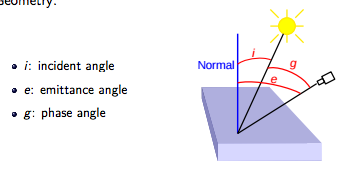
\includegraphics{images/brdf}
    \label{fig:brdf}
\end{figure}
\begin{itemize}
\item Bidirectional Reflectance Distribution Function
\item fraction of light reflected in the direction of the viewer
\item Lambertian: $\Phi(i,e,g) = \cos i$
\item Specular: $\Phi(i,e,g) = 1 $ when $ i = e $and$ g = i + e $
\item Largely property of the surface
\item Used in graphics a lot
\item Difficult to establish wavelength of light \& properties of surface
\item Determined experimentally
\end{itemize}

\paragraph{3D Surface information}

\textbf{Look up - 'Normal Mapping' wikipedia page}

Orientation of surface described by a normal vector (x,y,z):
\begin{itemize}
\item Change in z when x changes (p)
\item Change in z when y changes (q)
\end{itemize}

\subsubsection{Gradient Space}

$p = \dfrac{\delta z}{\delta x}$

$q = \dfrac{\delta z}{\delta y}$

\paragraph{Reflectance Map:}
\begin{itemize}
\item For surface of 'x' orientation, we expect this reflection back
\item[Light Change: ] 1 $=$ lightest, 0 $=$ darkest
\item Global solution found by integration in gradient and image space + smoothness assumption:
\begin{itemize}
\item Maths in confusing!
\item Don't need to know the maths for the exam
\end{itemize}
\end{itemize}


\subsubsection{Photometric Stereo}

We can reduce assumptions if we have multiple lighting conditions.

\textit{Example: 2 overlapping reflectance maps on sphere}

\begin{itemize}
\item Use same point in image plane under different lighting
\item You know where the lights are (calibrated)
\item Nothing moves - just the lights on/off
\item Calibration with sphere of similar reflectance
\item There is always noise
\item Reasonably robust
\end{itemize}

\textbf{This is at the heart of light-stage imaging}

\begin{itemize}
\item Illuminate with 1 source at a time
\item Calibrate \& results in look-up table
\end{itemize}

Have to reduce inter-reflections!

\paragraph{x,y,z mapped to RGB figures: }
\begin{itemize}
\item gives diagram of 3D structure
\end{itemize}

Fewer images $\rightarrow$ More assumptions

\textbf{$\star$ Look up ISO-contours}

\rule{\textwidth}{1pt}

\subsection{November 27: Shape from X}

\subsubsection{Shape from Texture}

1 + images, with a lot of assumptions.

\paragraph{Marr 1982:}
\begin{itemize}
\item 2 textured gradients
\item Limited information
\item Circles turn into ellipses (illusion of depth)
\end{itemize}

\paragraph{Types of textures:}
\begin{itemize}

\item[Isotropic:] rotation perpendicular to texture plane does not 'change' the texture
\item[Homogeneous:] texture looks 'the same' everywhere
\item[Texel:] basic texture elements, the repetition of which creates the texture
\end{itemize}

\paragraph{Local Binary Patterns}

\begin{itemize}
\item 3x3 filters
\item Capture changes in greyscale
\end{itemize}

\begin{figure}[h]
    \centering
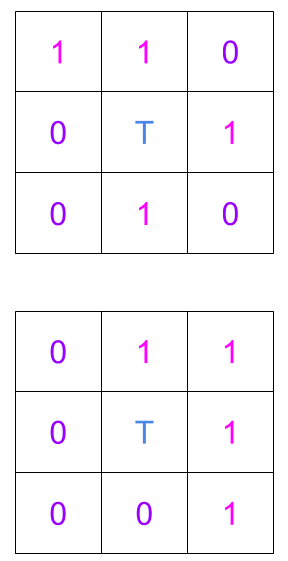
\includegraphics[scale=0.3]{images/local_binary}
\caption{Top: Standard output. Bottom: Could be used to detect edges}
    \label{fig:local_binary}
\end{figure}

0 $=$ darker than T
1 $=$ lighter than T

\paragraph{Global planes}
\begin{itemize}
\item Find the plane, uphill, downhill etc
\item Gradients in texture
\item Isotropic texture:
\begin{itemize}
\item circles $\rightarrow$ ellipses
\item Major axes of ellipses to work out slant \& tilt
\end{itemize}
\item Homogeneous texture:
\begin{itemize}
\item textures made of dots
\item look for a density change
\end{itemize}
\end{itemize}

Generally you fit methods locally rather than globally

\subsubsection{Shape from Motion}
Look up Marr (again)

Can also do structure from Motion: this is next week!

\textbf{The examples on BB are really good: biomotionlab!}

Things further away move more slowly - can infer things from this

\paragraph{Assumes:}
\begin{itemize}
\item rigidity 
\item parallel projection
\end{itemize}

Works both long and short range... 

\begin{itemize}
\item Initial guess on 3D model of world (flat screen)
\item + new image
\item update on those which disagree with the initial model
\end{itemize}

\textbf{Very popular!}

\subsubsection{Shape from Occlusions}
Infer shapes from which bits are in front of other parts

\paragraph{Occlusion contours:}
\begin{itemize}
\item discontinuity in depth signal
\item corresponds to silhouette (shadow)
\end{itemize}

\paragraph{Assumptions (1 image):}
\begin{itemize}
\item each point on contour corresponds to a single point on the object (except when a 'T' junction)
\item nearby points on the contour correspond to nearby points on the object
\item points on contour correspond to planar points on the object
\end{itemize}

\paragraph{When you have 2+ images:}
\begin{itemize}
\item Space Carving
\item Volumetric reconstruction
\item Gives where the object is \ isn't
\item Object is intersection of several generalised cones
\end{itemize}

\textbf{Watch the Youtube video on BB - Greenvision}

\begin{figure}[h]
    \centering
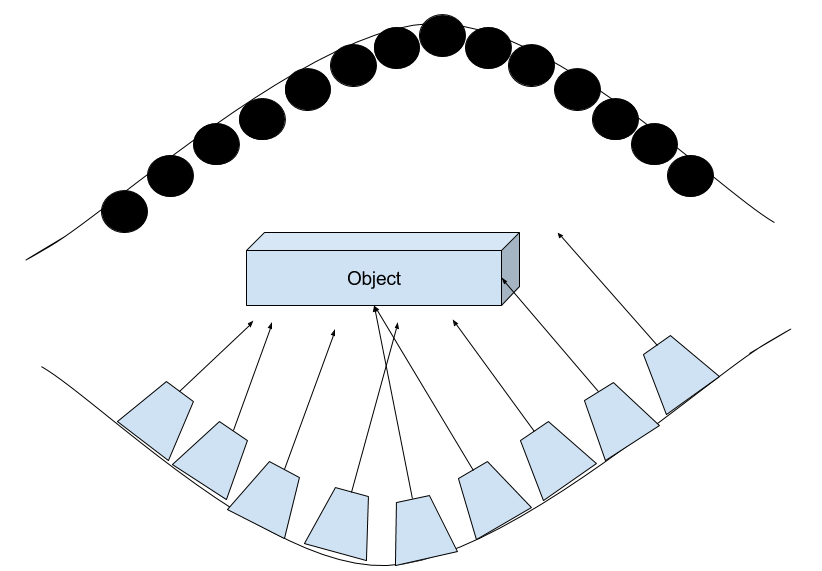
\includegraphics[scale=0.3]{images/occlusion}
\caption{Can the cameras see the points on the other side of the object? Make a map of what it can / can't see to build a shape of the object using multiple cameras (bottom row).}
    \label{fig:occlusion}
\end{figure}

\paragraph{From a video sequence:}
\begin{itemize}
\item inferred from motion \& occlusion
\item what occludes people in the scene?
\end{itemize}

Things at the front $=$ black, as it's never occluded from you 

Lots of motion $=$ white

\subsubsection{Shape from focal length}

\textit{Depth from defocus}

Things are blurry past a depth of focus
Take 10 pictures, at different lengths, with different focuses

\begin{itemize}
\item Texture really helps focus
\item Assumptions about smoothness
\end{itemize}

Markov-Random Field

\paragraph{How to tell if in focus?}
\begin{itemize}
\item Look for sharp edges $=$ \checkmark
\item Only low-frequency components $=$ \ding{55}
\end{itemize}

\rule{\textwidth}{1pt}

%-------------------------------------------------

\section{CS32310 - Advanced Computer Graphics}

%------------------------------------------------

\section{SE31520 - Internet-based Applications}


%------------------------------------------------

\section{Other}

%----------------------------------------------------------------------------------------

\end{document}